\section{Introduction}
\label{sec:introduction}

% state the learning objective 
The objective of this laboratory assignment is to study a circuit with four meshes containing a
voltage source $V_a$, a current source $I_d$, and two linearly dependent sources: a voltage controlled current source $I_b$ and a current controlled voltage source $V_c$. The circuit also contains seven Resistors from $R_1$ to $R_7$ as it is shown in Figure~\ref{fig:Circuit_Base}.
The values for the caracteristics of this components, apart of $I_b$ and $V_c$ and including $K_b$ and $K_c$, is given by python and are:

\begin{table}[h]
  \centering
  \begin{tabular}{|l|r|}
    \hline    
    {\bf Name} & {\bf Value [A, V, S or $\Omega$]} \\ \hline
    \#$R_{1}$ & 1.03258022265e+03 \\ \hline
\#$R_{2}$ & 2.05854281116e+03 \\ \hline
\#$R_{3}$ & 3.05658918951e+03 \\ \hline
\#$R_{4}$ & 4.12083818633e+03 \\ \hline
\#$R_{5}$ & 3.10223748153e+03 \\ \hline
\#$R_{6}$ & 2.09909352125e+03 \\ \hline
\#$R_{7}$ & 1.01569886691e+03 \\ \hline
  $V_{a}$ & 5.19832384287e+00 \\ \hline
 @$I_{d}$ & 1.04739543259e-03 \\ \hline
 §$K_{b}$ & 7.07448059081e-03 \\ \hline
\#$K_{c}$ & 8.22345657857e+03 \\ \hline

  \end{tabular}
  \caption{Variables in the Nodal Method. A variable preceded by @ is of type {\em current} and expressed in Ampere; variables preceded by \# is of type {\em resistance} and expressed in Ohm; variables preceded by § is of type {\em conductance} and expressed in Seimens; other variables are of type {\em voltage} and expressed in Volt.}
  \label{tab:Enunciado}
\end{table}

In Section~\ref{sec:analysis}, two different theoretical analysis of the circuit are
presented using the mesh method and the nodal method. In Section~\ref{sec:simulation}, the circuit is analysed by
simulation, and the results are compared to the theoretical ones obtained in
Section~\ref{sec:analysis}. The conclusions of this study are outlined in
Section~\ref{sec:conclusion}.

\begin{figure}[h] \centering
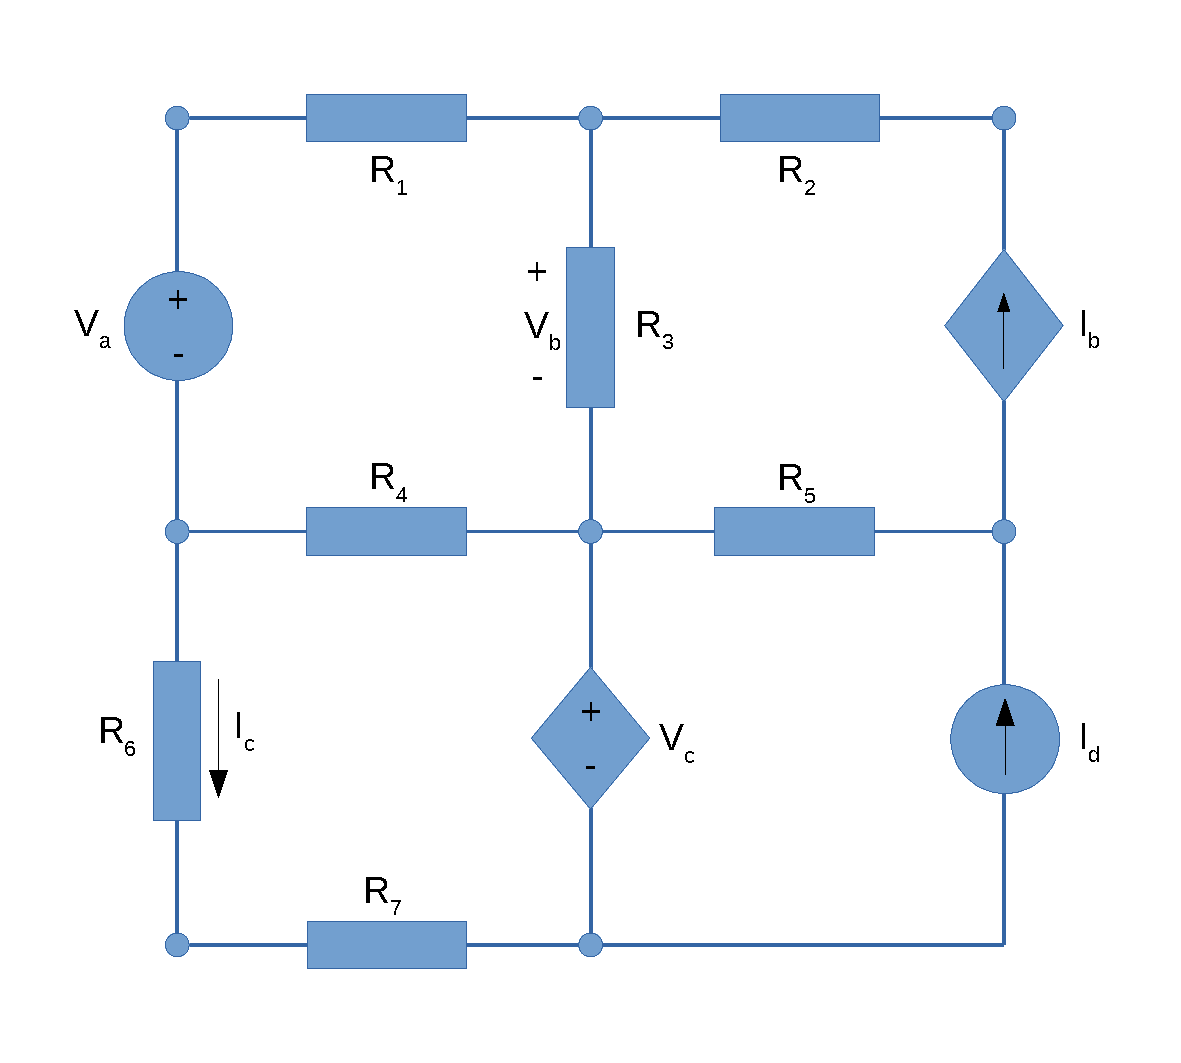
\includegraphics[width=0.5\linewidth]{Circuit.pdf}
\caption{Circuit analysed.}
\label{fig:Circuit_Base}
\end{figure}

